\documentclass[a4paper,12pt]{book}
\usepackage[utf8]{inputenc}
\usepackage{graphicx}
\graphicspath{{images/}}
\usepackage{listings}
\lstset{
	language=java,
	basicstyle=\sffamily,
	frame=none,
	breaklines=true,
	numbers=left,
	xleftmargin=1.8em,
	framexleftmargin=0em,
	emphstyle=\textbf,
	float=t
}
\lstdefinestyle{java}{
	basicstyle=\sffamily\small,
	emphstyle=\textbf,
	emph={
		public
		package, ., import, ;, @Entity, @IdClass, RateId, class,
		public, (, ), {, }, @Id, String, Double, this, =, return, SELECT, FROM, @Query, WHERE, DISTINCT,
		 <, >
	},
	commentstyle=\sffamily\textit,
	comment=[l]{\#}
}

\newcommand{\authors}[1]{{\chapterauthor{#1}\addtocontents{toc}{#1\par}}}

\renewcommand{\contentsname}{Daftar Isi}
\renewcommand{\chaptername}{Bab}
\renewcommand{\figurename}{Gambar}

\makeatletter
\newcommand{\chapterauthor}[1]{%
  {\parindent0pt\vspace*{-25pt}%
  \linespread{1.1}\large\scshape#1%
  \par\nobreak\vspace*{35pt}}
  \@afterheading%
}
\makeatother

\begin{document}

\title{Arsitektur Perangkat Lunak}
\author{Departemen Informatika, Universitas Pradita, Indonesia}
\date{2023}

\frontmatter
\maketitle
\tableofcontents

\mainmatter
\chapter{Pendahuluan}
\chapterauthor{Alfa Yohannis, Charlie Chaplin}

\section{Materi}
\begin{enumerate}
\item Introduction
\item Client-Server Architecture
\item Model-View-Controller Architecture
\item Model-View-ViewModel Architecture
\item Layered Architecture
\item Event-Driven Architecture
\item Pipeline / Pipe-and-Filter Architecture
\item Service-based (Serverless) Architecture
\item Microkernel Architecture
\item Space-based Architecture
\item Orchestration-driven Service-oriented Architecture
\item Microservices Architecture
\item Containers
\item DevOps
\end{enumerate}



\chapter{Pendahuluan}
\chapterauthor{Alfa Yohannis, Charlie Chaplin}

\section{Materi}
\begin{enumerate}
\item Introduction
\item Client-Server Architecture
\item Monolith vs. Distributed Architecture
\item Model-View-Controller Architecture
\item Layered Architecture
\item Event-Driven Architecture
\item Pipeline / Pipe-and-Filter Architecture
\item Service-based (Serverless) Architecture
\item Microkernel Architecture
\item Space-based Architecture
\item Orchestration-driven Service-oriented Architecture
\item Microservices Architecture
\item Containers
\item DevOps
\end{enumerate}



\chapter{Arsitektur MVC (Model-View-Controller)}
\authors{Alfa Yohannis}

\section{Latar Belakang}
Pada mulanya pengembangan perangkat lunak menyatukan fungsi-fungsi dari \textit{graphical user interface} (GUI) dan pengelolaan data ke dalam satu kode tanpa memisahkan mereka sesuai dengan perhatian (\textit{concerns}) mereka masing-masing. 
Konsekuensinya, pola tersebut akan menimbulkan masalah ketika \textit{developer} diminta untuk membangun aplikasi  skala besar,  misalnya aplikasi yang menolong pengguna berinteraksi dengan dataset yang besar dan kompleks. Kode program akan menjadi lebih tidak terstruktur (\textit{spaghetti code}) dan sulit untuk dipahami. 
Sebagai solusi, kode program perlu dibagi ke dalam komponen-komponen sesuai dengan perhatian mereka (\textit{separation of concerns}). 
Arsitektur Model-View-Controller (MVC) kemudian diajukan untuk membagi kode program ke dalam tiga abstraksi utama: \textit{model}, \textit{view}, dan \textit{controller}.

\section{Arsitektur Model-View-Controller}
Arsitektur MVC adalah pola arsitektur untuk pengembangan \textit{Graphical User Interface} (GUI). Arsitektur tersebut membagi logika progam menjadi 3 bagian yang saling terhubung: Model, View, dan Controller. Skema dari MVC dapat dilihat pada Gambar \ref{fig:mvc}..

\textbf{Model} ditujukan untuk berinteraksi dengan data: menyimpan, memperharui, menghapus, dan menarik data dari database. Model juga digunakan untuk menggagregasi data sesuai dengan logika bisnis yang dijalankan. 

\textbf{View} merupakan presentasi yang ditampilkan ke pengguna yang dengannya pengguna dapat berinteraksi. Misalnya, halaman web, GUI desktop, diagram, \textit{text fields}, \textit{buttons}, dsb.

\textbf{Controller} bertugas untuk menerima input dari pegguna melalui \textit{view} dan meneruskan input tersebut ke model untuk disimpan atau diproses lebih lanjut. Controller juga menarik data dari \textit{model} dan memembetuknya demikian rupa sehingga siap untuk dikirimkan ke \textit{view} untuk ditampilkan ke pengguna.

\begin{figure}[h]
    \centering
    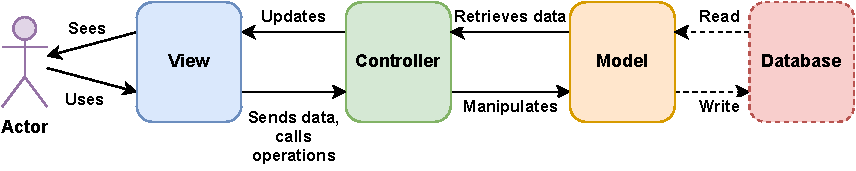
\includegraphics[width=\textwidth]{mvc}
    \caption{Arsitektur Model-View-Controller (MVC).}
    \label{fig:mvc}
\end{figure}

\section{Kelebihan dan Kekurangan}
Berikut adalah kelebihan dan kekurangan arsitektur MVC:


\subsection{Kelebihan}
Keuntungan dari menerapkan arsitektur MVC adalah:
\begin{itemize}
\item Pemisahan presentasi dan data membolehkan model ditampilkan di banyak \textit{view} secara bersamaan.
\item View bersifat \textit{composable} artinya view dapat dibangun dari berbagai atau berisi \textit{subviews}/\textit{fragments}.
\item Controller satu dapat diganti (\textit{switchable}) dengan controller lain pada saat \textit{runtime}.
\item Developer dapat membuat berbagai macam mekanisme pemrosesan data dari input ke output dengan mengkombinasikan berbagai macam fungsionalitas yang dimiliki oleh views, controllers, dan models.
\item \textit{Data engineers}, \textit{backend} dan \textit{frontend developers} masing-masing dapat fokus mengerjakan tugas utama mereka. 
Misal, \textit{data engineers} hanya mengerjakan tugas yang berkaitan dengan data, sendangkan \textit{frontend developers} fokus ke \textit{user interface}.
\end{itemize}

\subsection{Kekurangan}
Konsekuensi dari penerapan arsitektur MVC adalah sebagai berikut:
\begin{itemize}
\item Derajat kompleksitas kode program bertambah karena kode harus dibagi ke dalam tiga abstraksi yang berbeda.
\item \textit{Developers} harus mengikuti aturan ketat tertentu dalam mendefinisikan \textit{controllers}, \textit{models}, dan \textit{views}. 
\item Secara relative, MVC lebih sulit dipahami dikarenakan struktur bawaannya.
\item Terlalu berlebihan (\textit{overkill}) untuk aplikasi sederhana.
\item Cocok untuk pembangunan Graphical User Interface tetapi belum tentu cocok untuk pengembangan aplikasi atau komponen yang lain. 
\item Adanya lapisan-lapisan abstraksi dapat mengurangi kinerja (\textit{performance}) aplikasi.
\end{itemize}

\section{Contoh Kasus}

\subsection{Deskripsi}
Jelaskan contoh kasus yang dipaparkan berkaitan dengan arsitektur yang dimaksud pada bab ini.
Contoh kasus harus memperjelas arsitektur yang dimaksud.

\subsection{Penjelasan Implementasi}
Jelaskan bagian-bagian kode program, basisdata, atau konfigurasi yang signifikan terhadap arsitektur yang dimaksud.

\begin{lstlisting}[firstnumber=1,style=java,caption={Model dari \textsf{Rate}.},label=lst:rate_model]
import javax.persistence.Entity;
import javax.persistence.Id;
import javax.persistence.IdClass;

@Entity
@IdClass(RateId.class)
public class Rate {
  @Id
  private String fromCurrency;
  @Id
  private String toCurrency;
  private Double rate;
  ...
  Rate(String fromCurrency, String toCurrency, Double rate) {
    ...
  }
  ...
}
\end{lstlisting}

\begin{lstlisting}[firstnumber=1,style=java,caption={ \textsf{RateRepository}.},label=lst:rate_repository]
import java.util.Collection;
import org.springframework.data.jpa.repository.Query;
import org.springframework.data.repository.CrudRepository;

public interface RateRepository extends CrudRepository<Rate, Integer> {  
  @Query("SELECT r FROM Rate r WHERE r.fromCurrency = ?1 and r.toCurrency = ?2")
  Collection<Rate> findFirstByFromCurrencyAndToCurrency(String fromCurrency, String toCurrency);
  
  @Query("SELECT DISTINCT(r.fromCurrency) FROM Rate r")
  Collection<String> findAllFromCurrency();
  
  @Query("SELECT DISTINCT(r.toCurrency) FROM Rate r")
  Collection<String> findAllToCurrency(); 
}
\end{lstlisting}


\section{Kesimpulan}
Rangkum dan ulangi (beri penekanan pada) hal-hal kunci dari arsitektur yang dimaksud.
\chapter{Arsitektur MVC (Model-View-Controller)}
\authors{Alfa Yohannis}

\section{Latar Belakang}
Pada mulanya pengembangan perangkat lunak menyatukan fungsi-fungsi dari \textit{graphical user interface} (GUI) dan pengelolaan data ke dalam satu kode tanpa memisahkan mereka sesuai dengan perhatian (\textit{concerns}) mereka masing-masing. 
Konsekuensinya, pola tersebut akan menimbulkan masalah ketika \textit{developer} diminta untuk membangun aplikasi  skala besar,  misalnya aplikasi yang menolong pengguna berinteraksi dengan dataset yang besar dan kompleks. Kode program akan menjadi lebih tidak terstruktur (\textit{spaghetti code}) dan sulit untuk dipahami. 
Sebagai solusi, kode program perlu dibagi ke dalam komponen-komponen sesuai dengan perhatian mereka (\textit{separation of concerns}). 
Arsitektur Model-View-Controller (MVC) kemudian diajukan untuk membagi kode program ke dalam tiga abstraksi utama: \textit{model}, \textit{view}, dan \textit{controller}.

\section{Arsitektur Model-View-Controller}
Arsitektur MVC adalah pola arsitektur untuk pengembangan \textit{Graphical User Interface} (GUI). Arsitektur tersebut membagi logika progam menjadi 3 bagian yang saling terhubung: Model, View, dan Controller. Skema dari MVC dapat dilihat pada Gambar \ref{fig:mvc}..

\textbf{Model} ditujukan untuk berinteraksi dengan data: menyimpan, memperharui, menghapus, dan menarik data dari database. Model juga digunakan untuk menggagregasi data sesuai dengan logika bisnis yang dijalankan. 

\textbf{View} merupakan presentasi yang ditampilkan ke pengguna yang dengannya pengguna dapat berinteraksi. Misalnya, halaman web, GUI desktop, diagram, \textit{text fields}, \textit{buttons}, dsb.

\textbf{Controller} bertugas untuk menerima input dari pegguna melalui \textit{view} dan meneruskan input tersebut ke model untuk disimpan atau diproses lebih lanjut. Controller juga menarik data dari \textit{model} dan memembetuknya demikian rupa sehingga siap untuk dikirimkan ke \textit{view} untuk ditampilkan ke pengguna.

\begin{figure}[h]
    \centering
    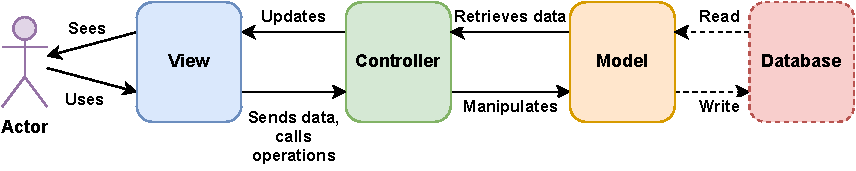
\includegraphics[width=\textwidth]{mvc}
    \caption{Arsitektur Model-View-Controller (MVC).}
    \label{fig:mvc}
\end{figure}

\section{Kelebihan dan Kekurangan}
Berikut adalah kelebihan dan kekurangan arsitektur MVC:


\subsection{Kelebihan}
Keuntungan dari menerapkan arsitektur MVC adalah:
\begin{itemize}
\item Pemisahan presentasi dan data membolehkan model ditampilkan di banyak \textit{view} secara bersamaan.
\item View bersifat \textit{composable} artinya view dapat dibangun dari berbagai atau berisi \textit{subviews}/\textit{fragments}.
\item Controller satu dapat diganti (\textit{switchable}) dengan controller lain pada saat \textit{runtime}.
\item Developer dapat membuat berbagai macam mekanisme pemrosesan data dari input ke output dengan mengkombinasikan berbagai macam fungsionalitas yang dimiliki oleh views, controllers, dan models.
\item \textit{Data engineers}, \textit{backend} dan \textit{frontend developers} masing-masing dapat fokus mengerjakan tugas utama mereka. 
Misal, \textit{data engineers} hanya mengerjakan tugas yang berkaitan dengan data, sendangkan \textit{frontend developers} fokus ke \textit{user interface}.
\end{itemize}

\subsection{Kekurangan}
Konsekuensi dari penerapan arsitektur MVC adalah sebagai berikut:
\begin{itemize}
\item Derajat kompleksitas kode program bertambah karena kode harus dibagi ke dalam tiga abstraksi yang berbeda.
\item \textit{Developers} harus mengikuti aturan ketat tertentu dalam mendefinisikan \textit{controllers}, \textit{models}, dan \textit{views}. 
\item Secara relative, MVC lebih sulit dipahami dikarenakan struktur bawaannya.
\item Terlalu berlebihan (\textit{overkill}) untuk aplikasi sederhana.
\item Cocok untuk pembangunan Graphical User Interface tetapi belum tentu cocok untuk pengembangan aplikasi atau komponen yang lain. 
\item Adanya lapisan-lapisan abstraksi dapat mengurangi kinerja (\textit{performance}) aplikasi.
\end{itemize}

\section{Contoh Kasus}

\subsection{Deskripsi}
Jelaskan contoh kasus yang dipaparkan berkaitan dengan arsitektur yang dimaksud pada bab ini.
Contoh kasus harus memperjelas arsitektur yang dimaksud.

\subsection{Penjelasan Implementasi}
Jelaskan bagian-bagian kode program, basisdata, atau konfigurasi yang signifikan terhadap arsitektur yang dimaksud.

\begin{lstlisting}[firstnumber=1,style=java,caption={Model dari \textsf{Rate}.},label=lst:rate_model]
import javax.persistence.Entity;
import javax.persistence.Id;
import javax.persistence.IdClass;

@Entity
@IdClass(RateId.class)
public class Rate {
  @Id
  private String fromCurrency;
  @Id
  private String toCurrency;
  private Double rate;
  ...
  Rate(String fromCurrency, String toCurrency, Double rate) {
    ...
  }
  ...
}
\end{lstlisting}

\begin{lstlisting}[firstnumber=1,style=java,caption={ \textsf{RateRepository}.},label=lst:rate_repository]
import java.util.Collection;
import org.springframework.data.jpa.repository.Query;
import org.springframework.data.repository.CrudRepository;

public interface RateRepository extends CrudRepository<Rate, Integer> {  
  @Query("SELECT r FROM Rate r WHERE r.fromCurrency = ?1 and r.toCurrency = ?2")
  Collection<Rate> findFirstByFromCurrencyAndToCurrency(String fromCurrency, String toCurrency);
  
  @Query("SELECT DISTINCT(r.fromCurrency) FROM Rate r")
  Collection<String> findAllFromCurrency();
  
  @Query("SELECT DISTINCT(r.toCurrency) FROM Rate r")
  Collection<String> findAllToCurrency(); 
}
\end{lstlisting}


\section{Kesimpulan}
Rangkum dan ulangi (beri penekanan pada) hal-hal kunci dari arsitektur yang dimaksud.
\chapter{Layered Architecture}
\authors{Austin Nicholas Tham, Darren Valentio, Muhammad}

%%Tolong tambahkan daftar gambar contoh : Gambar 5.1, 5.2, dst.. dan tambahkan italic text untuk setiap bahasa asing
%%Regards, Glenny ^^.

\section{Definisi \textit{Layered Architechture}}

Pola arsitektur layered adalah pola n-tiered di mana komponen disusun dalam lapisan horizontal. Ini adalah metode tradisional untuk merancang sebagian besar perangkat lunak dan dimaksudkan untuk pengembangan mandiri sehingga semua komponen saling berhubungan tetapi tidak saling bergantung.

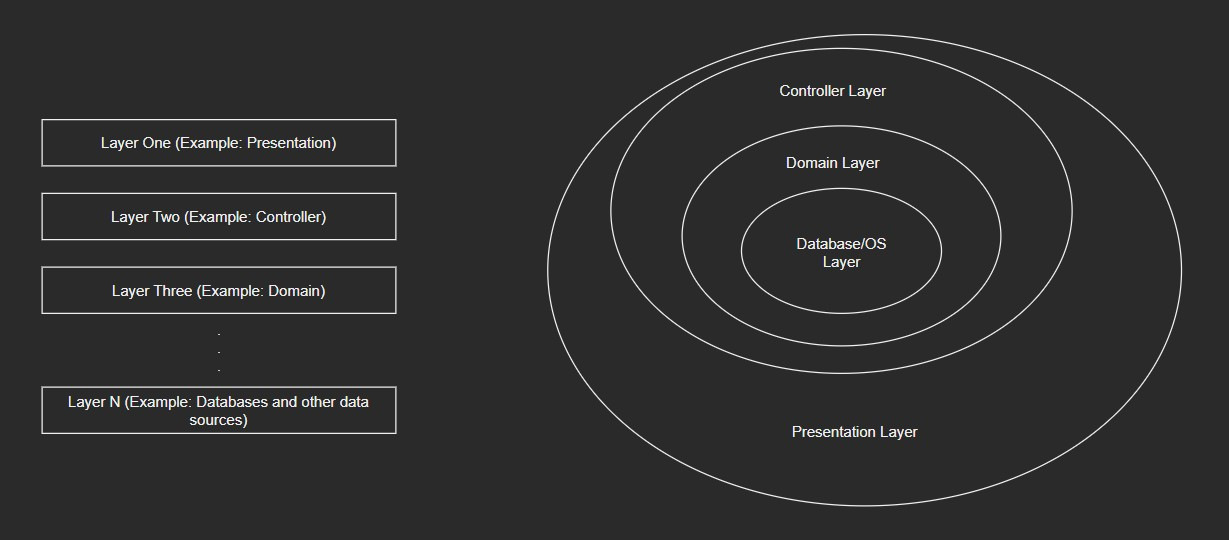
\includegraphics[width=\textwidth]{../images/chapter05/Layering Architecture}

Seperti yang ditunjukkan pada gambar, layering biasanya dilakukan dengan mengemas fungsionalitas khusus aplikasi di lapisan atas, penyebaran fungsionalitas spesifik menjadi lapisan bawah dan fungsionalitas yang membentang di seluruh domain aplikasi di lapisan tengah. Jumlah lapisan dan bagaimana lapisan-lapisan ini disusun ditentukan oleh kompleksitas masalah dan solusinya.

Di sebagian besar arsitektur berlapis, ada beberapa lapisan (atas ke bawah):

\begin{itemize}
    \item \textbf{The application layered:} Berisi layanan spesifik aplikasi.
    \item \textbf{The business layer:} Menangkap komponen yang umum di beberapa aplikasi.
    \item \textbf{The middleware layer:} Lapisan ini mengemas beberapa fungsi seperti pembangun GUI, antarmuka ke basis data, laporan, dan dll.
    \item \textbf{The database/System Software Layer:} Berisi OS, database, dan antarmuka ke komponen perangkat keras tertentu.
\end{itemize}

\section{Latar Belakang}

Penilaian untuk setiap karakteristik berdasarkan kecenderungan alami untuk implementasi tipikal pola layered.

\begin{itemize}
    \item Kemampuan untuk merespon dengan cepat terhadap lingkungan yang terus berubah. (monolitik)
    \item Bergantung pada implementasi pola, penyebaran bisa menjadi masalah. Satu perubahan kecil ke komponen dapat memerlukan redeployment seluruh aplikasi.
    \item Pengembang dapat memberikan pengujian singkat untuk menguji aplikasi sebelum klien menggunakannya
    \item Mudah dikembangkan karena polanya sudah terkenal dan tidak terlalu rumit untuk melakukan implementasinya.
\end{itemize}

\section{Pros Cons}

\subsection{Pros}

\begin{itemize}
    \item Mudah untuk diuji karena komponen-komponennya termasuk lapisan khusus sehingga dapat diuji secara terpisah.
    \item Sederhana dan mudah diimplementasikan karena secara alami, sebagian besar aplikasi bekerja berlapis-lapis
\end{itemize}

\subsection{Cons}

\begin{itemize}
    \item Tidak mudah untuk melakukan perubahan pada lapisan tertentu karena aplikasi merupakan unit tunggal.
    \item Kopling antar lapisan cenderung membuatnya lebih sulit. Hal ini membuatnya sulit untuk diukur.
    \item Harus digunakan sebagai unit tunggal sehingga perubahan ke lapisan tertentu berarti seluruh sistem harus dipekerjakan kembali.
    \item Semakin besar, semakin banyak sumber daya yang dibutuhkan untuk permintaan untuk melewati beberapa lapisan dan dengan demikian akan menyebabkan masalah kinerja.
\end{itemize}

\section{Software Architechture Pattern}
Ini adalah pola arsitektur paling umum di sebagian besar aplikasi tingkat perusahaan. Ini juga dikenal sebagai pola n-tier, dengan asumsi n jumlah tingkatan. Contoh Skenario:

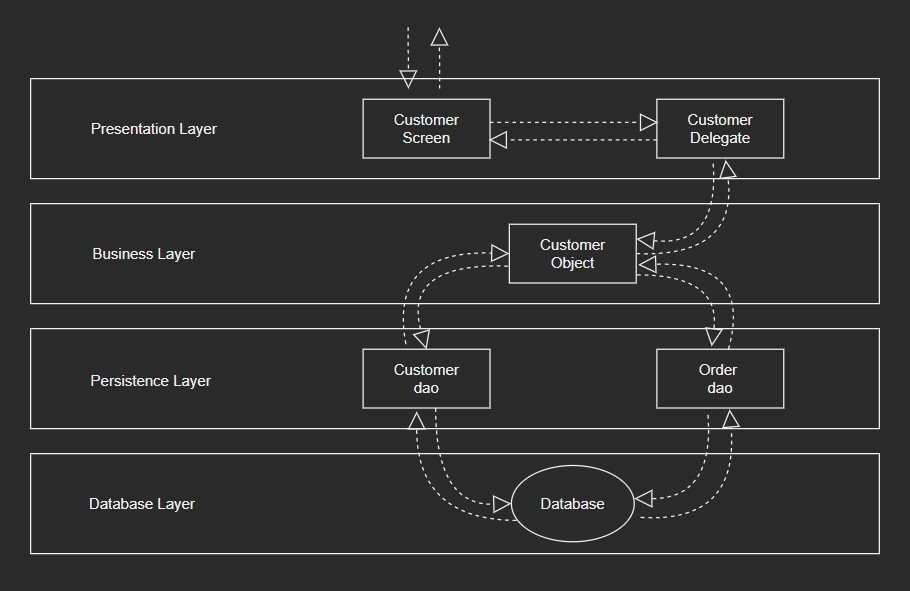
\includegraphics[width=\textwidth]{../images/chapter05/Software Architecture Pattern}


\section{Design Patterns}

Anggap mock-up software design, susunan “stack” nya seperti layered architecture:

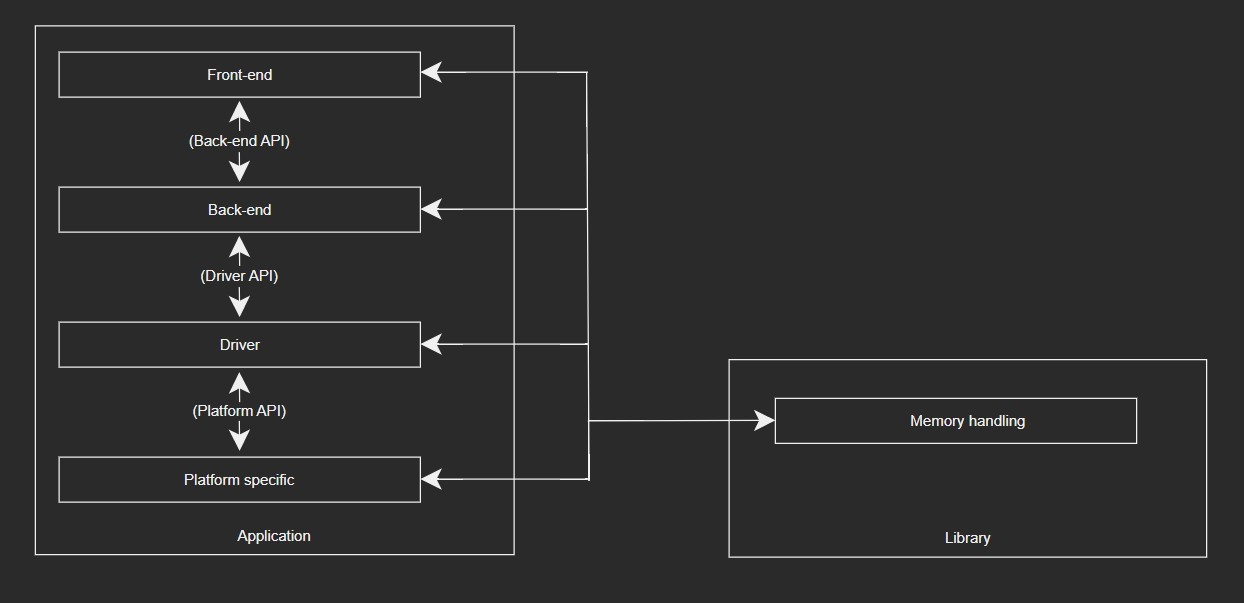
\includegraphics[width=\textwidth]{../images/chapter05/Design Pattern}

Setiap layer dari aplikasi terpisah dengan cara penggunaan metode API, namun yang masih saling berhubungan adalah memory handling , karena setiap komunikasi layer akan membawa/mengirim data sehingga akan terjadi alokasi memory dan pada akhirnya membutuhkan memory handling.

Ada 4 bagian dari layered architecture yang di mana setiap layer memiliki hubungan antara komponen yang ada di dalamnya dari atas ke bawah yaitu:

\begin{itemize}
    \item \textbf{The presentation layer:} Semua bagian yang berhubungan dengan layer presentasi.
    \item \textbf{The business layer:} Berhubungan dengan logika bisnis.
    \item \textbf{The persistence layer:} Berguna untuk mengurusi semua fungsi yang berhubungan dengan objek relasional
    \item \textbf{The database layer:} Tempat penyimpanan semua data layer.
\end{itemize}

\subsection{Contoh penerapan layered architecture:}

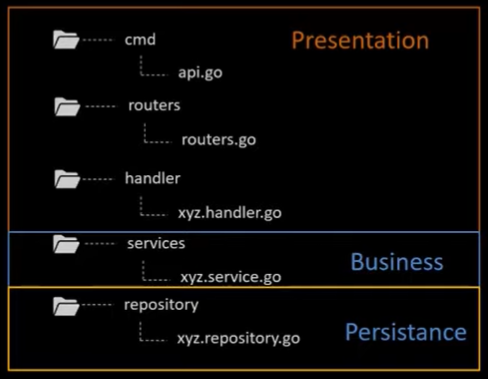
\includegraphics[width=\textwidth]{../images/chapter05/contoh}


\chapter{Pendahuluan}
\chapterauthor{Alfa Yohannis, Charlie Chaplin}

\section{Materi}
\begin{enumerate}
\item Introduction
\item Client-Server Architecture
\item Monolith vs. Distributed Architecture
\item Model-View-Controller Architecture
\item Layered Architecture
\item Event-Driven Architecture
\item Pipeline / Pipe-and-Filter Architecture
\item Service-based (Serverless) Architecture
\item Microkernel Architecture
\item Space-based Architecture
\item Orchestration-driven Service-oriented Architecture
\item Microservices Architecture
\item Containers
\item DevOps
\end{enumerate}



\chapter{Pendahuluan}
\chapterauthor{Alfa Yohannis, Charlie Chaplin}

\documentclass{article}
\usepackage{indentfirst}
\setlength{\parskip}{20pt}
\usepackage[utf8]{inputenc}
\usepackage{graphicx}
\graphicspath{{images/}}
\usepackage{varwidth}

\begin{document}
	\begin{titlepage}
		\begin{center}
			\textbf{\huge Pipe and Filter}
			
			\vspace{0.5cm}
				
			{\large Software Architecture}
			
			\vspace{2.5cm}
			
			\section*{Nama}
			\begin{varwidth}{\textwidth}
				\begin{itemize}
					\item Wahyudi 2110101022
					\item Tommy Chitiawan 2110101025
					\item Mandalan 2110101028
				\end{itemize}
			\end{varwidth}

			
			
		\end{center}

	\end{titlepage}
	\section{Definisi}
	Pipa dan Filter adalah pola arsitektur lain, yang memiliki entitas independen yang disebut filter (komponen) yang melakukan transformasi pada data dan memproses masukan yang mereka terima, dan pipa , yang berfungsi sebagai penghubung aliran data yang sedang diubah, masing-masing terhubung ke komponen berikutnya di dalam pipa.
	
	\section{Pipe and Filter Architecture Schema
	}
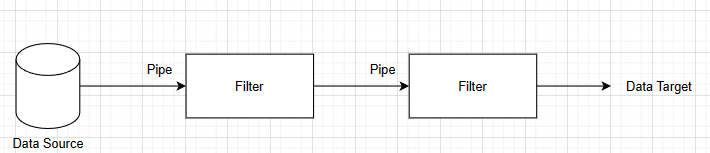
\includegraphics{Capture.png}

	\section{Kelebihan}
	
	\begin{itemize}
		\item Memastikan sambungan komponen, filter yang longgar dan fleksibel.
		\item Kopling longgar memungkinkan filter diubah tanpa modifikasi ke filter lain.
		\item Konduktif untuk pemrosesan paralel.
		\item Filter dapat diperlakukan sebagai kotak hitam. Pengguna sistem tidak perlu mengetahui logika di balik kerja setiap filter.
		\item Dapat digunakan kembali. Setiap filter dapat dipanggil dan digunakan berulang kali.
	\end{itemize}
.
	
	
	\section{Kekurangan}
	
	\begin{itemize}
		\item 	Penambahan sejumlah besar filter independen dapat mengurangi kinerja karena overhead komputasi yang berlebihan.
		\item Bukan pilihan yang baik untuk sistem interaktif.
		\item Sistem pipa-dan-pemasang mungkin tidak cocok untuk perhitungan jangka panjang.
		
	\section{penerapan dalam aplikasi}
	\begin{itemize}
		\item Sistem pengolahan data: Pipe and filter dapat digunakan untuk mengambil data dari berbagai sumber dan memprosesnya melalui serangkaian filter untuk menghasilkan output yang diinginkan.
			
		\item Sistem pengolahan gambar: Pipe and filter dapat digunakan untuk memproses gambar atau video yang diambil dari kamera dengan menggunakan berbagai filter untuk menghasilkan gambar yang lebih baik atau memberikan efek khusus.
			
		\item Sistem pencarian: Pipe and filter dapat digunakan untuk memproses data pencarian yang diberikan oleh pengguna dan memfilter data untuk menghasilkan hasil pencarian yang relevan.
			
		\item Sistem pemrosesan audio: Pipe and filter dapat digunakan untuk memproses audio dan melakukan pengolahan suara seperti pengurangan kebisingan, pengaturan volume, dan pemotongan audio.
			
		\item Sistem pemrosesan teks: Pipe and filter dapat digunakan untuk memproses teks dan melakukan pengolahan bahasa alami seperti analisis sentimen dan pengenalan entitas.
			content...
		\end{itemize}
	\end{itemize}
\end{document}


\chapter{Serverless Architecture}
\authors{Ryan Christensen Wang, Steven Tanaka, Yogi Valentino Nadeak}

	\gny{Tolong tambahkan keterangan gambar contoh : Gambar 8.1, 8.2, dst.. dan tambahkan italic text untuk setiap bahasa asing}
	
\section{Definisi Serverless Architechture}
Serverless architecture merupakan pendekatan dalam desain software yang mana developer tidak perlu pusing-pusing lagi mengelola infrastruktur seperti server.Developer bisa fokus dalam mengembangkan aplikasinya dan masalah server akan dikelola oleh penyedia layanan serverless (provider).

Less dalam serverless bukan berarti tanpa server sama sekali, tetapi memungkinkan untuk konfigurasi seminimal mungkin atau dikurangi. Misalnya, pengembang tidak perlu tidak perlu otak-atik konfigurasi web server ketika melakukan deploy kode yang hanya tinggal dihubungkan ke proxy.

Developer menggunakan Serverless Architecture untuk menggunakan kembali layanan dalam sistem yang berbeda atau menggabungkan beberapa layanan independen untuk melakukan tugas yang kompleks. 

Misalnya, beberapa proses bisnis dalam suatu organisasi memerlukan fungsionalitas autentikasi pengguna. Alih-alih menulis ulang kode autentikasi untuk semua proses bisnis, Anda dapat membuat satu layanan autentikasi dan menggunakannya kembali untuk semua aplikasi. Demikian juga dengan sistem di seluruh organisasi layanan kesehatan, seperti sistem manajemen pasien dan sistem catatan kesehatan elektronik (EHR), sebagian besar perlu mendaftarkan pasien. Sistem ini dapat memanggil satu layanan umum untuk melakukan tugas pendaftaran pasien.

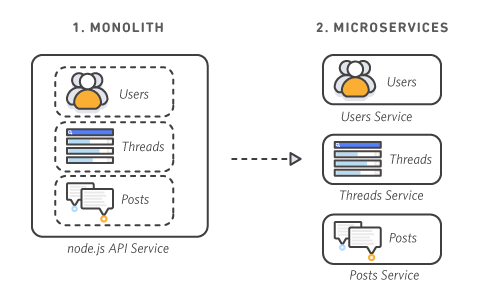
\includegraphics[width=\textwidth]{Mono.png}

\textbf{Ada beberapa istilah dasar dalam arsitektur ini, antara lain:}

\begin{itemize}
	\item \textbf{Invocation,} yaitu eksekusi fungsi tunggal.
	\item \textbf{Duration,} durasi waktu yang dibutuhkan fungsi serverless
	\item \textbf{Cold start,} yaitu terjadinya latensi saat fungsi ter-trigger pertama kali atau setelah periode tidak aktif.
	\item \textbf{Concurrency limit,} yaitu jumlah fungsi instance yang dapat dijalankan secara bersamaan dalam satu wilayah
	\item \textbf{Timeout,} yaitu jumlah waktu yang diizinkan oleh penyedia layanan untuk menjalankan fungsi sebelum dihentikan.
\end{itemize}

Serverless architecture ini cocok digunakan untuk kasus yang melakukan tugas jangka pendek dan mengelola beban kerja yang mengalami lalu lintas yang jarang dan tidak dapat diprediksi. Ada beberapa kasus lain yang dapat dipertimbangkan menggunakan arsitektur ini, yaitu:

\begin{itemize}
	\item Tugas yang berdasarkan trigger
	\item Membangun RESTful API
	\item Continuous Integration dan Continuous Delivery (CI/CD)
	\item Proses asinkronus
\end{itemize}

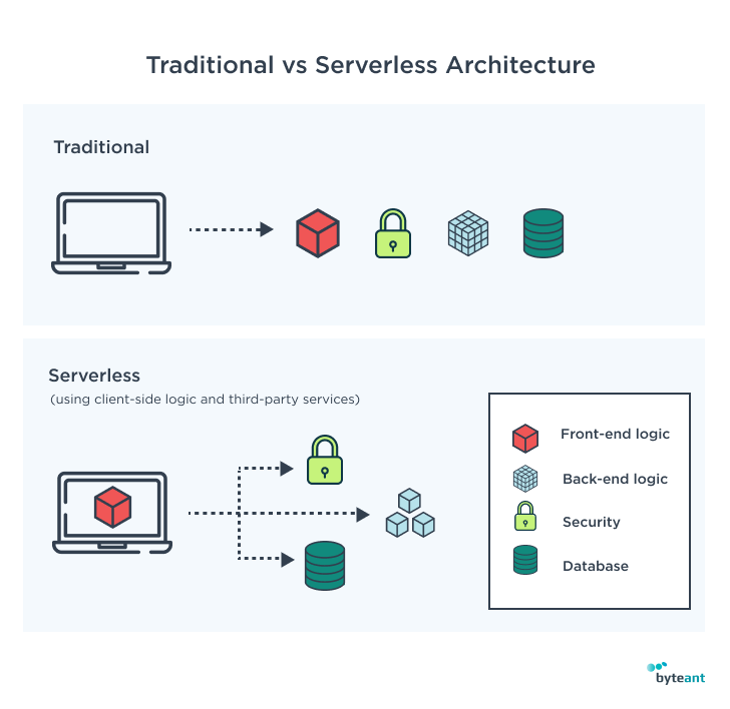
\includegraphics[width=\textwidth]{Archi.png}

\section{Fungsi/Kegunaan dari Serverless Architecture}

Serverless architecture adalah sebuah model komputasi di awan yang mana penyedia layanan awan bertanggung jawab dalam mengelola infrastruktur dan memperuntukan sumber daya komputasi yang dibutuhkan secara otomatis, tanpa pengguna perlu mengurus atau merawat server. Terdapat beberapa keuntungan dari penggunaan arsitektur serverless, diantaranya adalah:

Penilaian untuk setiap karakteristik berdasarkan kecenderungan alami untuk implementasi tipikal pola layered.

\begin{itemize}
	\item optimisasi biaya dengan hanya membayar untuk sumber daya yang digunakan
	\item memungkinkan pengembangan aplikasi yang lebih cepat
	\item skalabilitas yang mudah untuk mengakomodasi perubahan permintaan
	\item serta perawatan dan pemeliharaan yang lebih mudah karena dikelola oleh penyedia layanan awan.
\end{itemize}

\section{Kekurangan dan Kelebihan dari Serverless Architecture}
\subsection{Kelebihan dari Serverless Architecture}

\begin{itemize}
	\item \textbf{Skalabilitas:} Dalam arsitektur serverless, aplikasi dapat dengan mudah ditingkatkan kapasitasnya untuk menangani permintaan yang berfluktuasi, sehingga dapat mengurangi pengeluaran untuk infrastruktur yang tidak terpakai.
	\item \textbf{Biaya operasional yang rendah:} Dalam serverless, pengguna hanya membayar untuk sumber daya yang mereka gunakan, yang dapat mengurangi biaya operasional secara signifikan.
	\item \textbf{Fokus pada pengembangan aplikasi:} Dalam serverless, pengembang tidak perlu khawatir mengurus infrastruktur server dan dapat fokus pada pengembangan aplikasi.
	\item \textbf{Perawatan dan pemeliharaan yang mudah:} Dalam serverless, penyedia layanan awan bertanggung jawab atas perawatan dan pemeliharaan infrastruktur, sehingga pengguna tidak perlu memikirkan pembaruan sistem operasi atau patch keamanan.
\end{itemize}

\subsection{Kekurangan dari Serverless Architecture}

\begin{itemize}
	\item \textbf{Keterbatasan dalam penggunaan:} Serverless mungkin tidak cocok untuk semua jenis aplikasi, terutama jika aplikasi memerlukan kontrol tinggi atas infrastruktur dan lingkungan di mana aplikasi berjalan.
	\item \textbf{Ketergantungan pada penyedia layanan awan:} Serverless membuat pengguna sangat bergantung pada penyedia layanan awan, sehingga jika terjadi masalah atau gangguan pada layanan, aplikasi dapat mengalami downtime yang signifikan.
	\item \textbf{Pengaturan konfigurasi yang kompleks:} Serverless dapat memiliki konfigurasi yang kompleks dan memerlukan pengaturan yang cermat untuk memastikan aplikasi berjalan dengan baik.
	\item \textbf{Performa yang tidak stabil:} : Serverless dapat mengalami performa yang tidak stabil jika pengguna tidak melakukan penyesuaian yang cermat dalam skala dan konfigurasi aplikasi.
\end{itemize}

\section{Penerapan Serverless Architecture}
	Serverless Architecture adalah model komputasi awan di mana penyedia awan secara dinamis mengelola alokasi dan penyediaan server, memungkinkan pengembang untuk fokus menulis kode tanpa harus mengelola infrastruktur.
	
	Berikut adalah beberapa contoh penerapan serverless architecture:
	\begin{itemize}
		\item \textbf{Web applications:} Pengembang dapat membangun dan menerapkan aplikasi web menggunakan arsitektur tanpa server, tanpa harus mengelola server atau infrastruktur. Mereka dapat menggunakan layanan seperti AWS Lambda, Google Cloud Functions, atau Azure Functions untuk menulis kode yang merespons kejadian, seperti permintaan HTTP, dan berjalan sesuai permintaan.
		\item \textbf{Data processing:} Serverless Architecture dapat digunakan untuk tugas pemrosesan data seperti transformasi data, pembersihan, dan analisis. Pengembang dapat menggunakan layanan seperti AWS Glue, Google Cloud Dataflow, atau Azure Stream Analytics untuk memproses data tanpa server, tanpa harus mengelola server atau infrastruktur.
		\item \textbf{Chatbots:} Pengembang dapat membangun chatbot menggunakan serverless, dengan menulis kode yang merespons acara obrolan, seperti pesan pengguna. Mereka dapat menggunakan layanan seperti AWS Lex, Google Cloud Dialogflow, atau Azure Bot Service untuk membuat dan menerapkan chatbot yang berjalan sesuai permintaan.
		\item \textbf {IoT applications:} Serverless Architecture dapat digunakan untuk aplikasi IoT, dengan memungkinkan pengembang menulis kode yang merespons kejadian dari perangkat IoT, seperti pembacaan sensor. Mereka dapat menggunakan layanan seperti AWS IoT, Google Cloud IoT Core, atau Azure IoT Hub untuk membangun dan menerapkan aplikasi IoT tanpa server.
	\end{itemize}



\chapter{Pendahuluan}
\chapterauthor{Alfa Yohannis, Charlie Chaplin}

\section{Materi}
\begin{enumerate}
\item Introduction
\item Client-Server Architecture
\item Monolith vs. Distributed Architecture
\item Model-View-Controller Architecture
\item Layered Architecture
\item Event-Driven Architecture
\item Pipeline / Pipe-and-Filter Architecture
\item Service-based (Serverless) Architecture
\item Microkernel Architecture
\item Space-based Architecture
\item Orchestration-driven Service-oriented Architecture
\item Microservices Architecture
\item Containers
\item DevOps
\end{enumerate}



\chapter{Pendahuluan}
\chapterauthor{Alfa Yohannis, Charlie Chaplin}

\section{Materi}
\begin{enumerate}
\item Introduction
\item Client-Server Architecture
\item Monolith vs. Distributed Architecture
\item Model-View-Controller Architecture
\item Layered Architecture
\item Event-Driven Architecture
\item Pipeline / Pipe-and-Filter Architecture
\item Service-based (Serverless) Architecture
\item Microkernel Architecture
\item Space-based Architecture
\item Orchestration-driven Service-oriented Architecture
\item Microservices Architecture
\item Containers
\item DevOps
\end{enumerate}



\chapter{Orchestration-driven Service-oriented Architecture}
\authors{Hansel Ricardo, Jonathan Erik Maruli Tua, Yefta Tanuwijaya}

% Tolong tambahkan keterangan gambar contoh : Gambar 11.1, 11.2, dst.. dan tambahkan italic text untuk setiap bahasa asing

\section{Definisi}
\textit{Orchestration-driven Service-oriented Architecture} (ODSOA) adalah suatu pendekatan arsitektur perangkat lunak yang bertujuan untuk memfasilitasi pengembangan dan integrasi sistem yang kompleks dengan cara menggunakan layanan (\textit{Services}) yang terdistribusi dan terpisah secara fisik namun saling terkait secara fungsional.

ODSOA menempatkan Orkestrasi (\textit{Orchestration}) sebagai elemen kunci untuk mengelola interaksi antara layanan. Orkestrasi dapat didefinisikan sebagai proses otomatis yang mengkoordinasikan dan mengatur eksekusi layanan secara teratur untuk mencapai tujuan bisnis tertentu.

Dalam ODSOA, layanan disediakan sebagai fungsi-fungsi modular yang dapat digunakan oleh aplikasi dan sistem lain untuk memperoleh fungsionalitas tambahan. Layanan ini biasanya disediakan secara independen oleh unit bisnis atau departemen yang berbeda dan dapat diakses melalui jaringan.

ODSOA memiliki beberapa keuntungan, antara lain: skalabilitas, fleksibilitas, dan interoperabilitas. Skalabilitas memungkinkan sistem untuk diukur dan meningkatkan kapasitasnya dengan mudah. Fleksibilitas memungkinkan pengguna untuk menyesuaikan layanan sesuai kebutuhan mereka tanpa harus mengubah keseluruhan arsitektur. Interoperabilitas memungkinkan sistem untuk berinteraksi dengan sistem lain yang menggunakan standar yang sama.

Secara keseluruhan, ODSOA dapat membantu perusahaan dalam mempercepat pengembangan dan integrasi aplikasi serta meningkatkan efisiensi dan efektivitas bisnis secara keseluruhan.
	
\section{\textit{Orchestration-driven Service-oriented Architecture Schema}}

\begin{figure}[h]
	\centering
	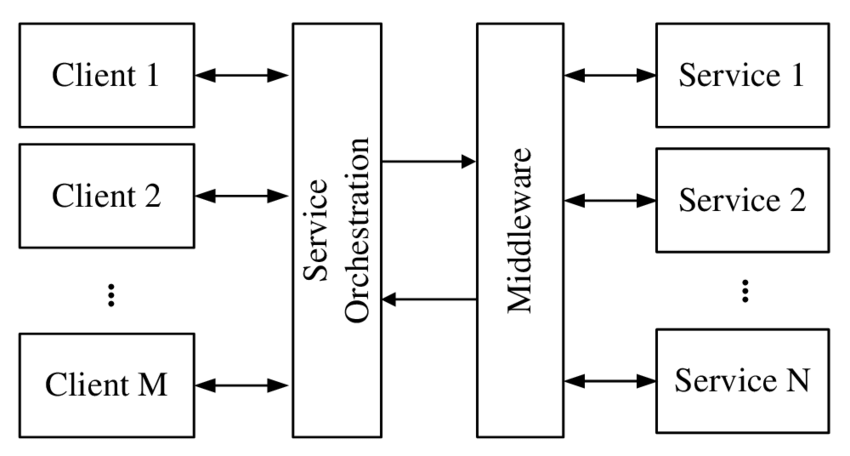
\includegraphics[width=\textwidth]{ODSOA}
	\caption {Arsitektur ODSOA.}
	\label{fig:Arsitektur ODSOA}
\end{figure}

\textit{Orchestration-driven Service-oriented Architecture} (ODSOA) Schema adalah suatu model yang menggambarkan arsitektur ODSOA secara visual, yang mencakup komponen-komponen utama dan interaksi antara mereka. Beberapa komponen utama dalam schema ODSOA antara lain:
	\begin{itemize}
	\item Layanan (\textit{Services}): Komponen inti dari ODSOA adalah layanan, yang merupakan unit fungsional yang terdistribusi secara terpisah namun saling terkait secara fungsional. Layanan ini dapat digunakan oleh aplikasi dan sistem lain untuk memperoleh fungsionalitas tambahan.
	\item Orkestrasi (\textit{Orchestration}): Orkestrasi merupakan proses otomatis yang mengkoordinasikan dan mengatur eksekusi layanan secara teratur untuk mencapai tujuan bisnis tertentu. Orkestrasi dapat mengatur urutan dan kondisi yang harus dipenuhi oleh layanan.
	\item Bus Layanan (\textit{Service Bus}): Bus Layanan adalah infrastruktur yang memfasilitasi komunikasi antara layanan dalam arsitektur ODSOA. Bus Layanan dapat mengatur dan mengarahkan permintaan dan respons antara layanan.
	\item Repositori Layanan (\textit{Service Repository}): Repositori Layanan adalah tempat untuk menyimpan informasi terkait dengan layanan yang tersedia, seperti deskripsi, spesifikasi teknis, dan interdependensi antara layanan. Repositori Layanan memungkinkan pengguna untuk mencari dan menemukan layanan yang dibutuhkan.
	\item Klien (\textit{Client}): Klien adalah aplikasi atau sistem yang menggunakan layanan untuk memperoleh fungsionalitas tambahan. Klien mengirim permintaan ke layanan dan menerima respons dari layanan.
	\item Penyedia Layanan (\textit{Service Provider}): Penyedia Layanan adalah unit bisnis atau departemen yang menyediakan layanan untuk digunakan oleh aplikasi dan sistem lain. Penyedia Layanan bertanggung jawab untuk mengembangkan dan menjaga layanan yang disediakan.
	\end{itemize}
Dalam ODSOA Schema, interaksi antara komponen-komponen tersebut direpresentasikan dengan panah yang menghubungkan mereka. Misalnya, panah dari klien ke layanan menunjukkan bahwa klien menggunakan layanan tersebut, sedangkan panah dari layanan ke bus layanan menunjukkan bahwa layanan terdaftar dalam infrastruktur bus layanan. Dengan ODSOA Schema, pengguna dapat dengan mudah memahami arsitektur ODSOA secara visual dan mengidentifikasi komponen-komponen utama dan interaksi antara mereka.

\section{Kelebihan}
\begin{itemize}
\item Skalabilitas: ODSOA memungkinkan sistem untuk diukur dan meningkatkan kapasitasnya dengan mudah. Layanan dapat dikonfigurasi ulang atau ditambahkan ke infrastruktur dengan mudah, tanpa mempengaruhi sistem keseluruhan. Hal ini memudahkan perusahaan untuk menyesuaikan sistem mereka dengan perubahan kebutuhan bisnis.
\item Fleksibilitas: ODSOA memungkinkan pengguna untuk menyesuaikan layanan sesuai kebutuhan mereka tanpa harus mengubah keseluruhan arsitektur. Dengan demikian, perusahaan dapat dengan mudah memodifikasi fungsionalitas sistem dan mengintegrasikan solusi baru tanpa mempengaruhi sistem keseluruhan.
\item Interoperabilitas: ODSOA memungkinkan sistem untuk berinteraksi dengan sistem lain yang menggunakan standar yang sama. Hal ini memungkinkan perusahaan untuk berintegrasi dengan sistem lain dengan mudah dan memperluas fungsionalitas sistem mereka.
\item Reusabilitas: Layanan dalam ODSOA adalah modular dan dapat digunakan kembali oleh aplikasi dan sistem lain. Hal ini memungkinkan perusahaan untuk mengembangkan sistem dengan cepat dan efisien.
\item Pemisahan Tugas: ODSOA memisahkan tugas-tugas sistem menjadi layanan yang terpisah secara fisik namun saling terkait secara fungsional. Hal ini memudahkan manajemen sistem dan memungkinkan perusahaan untuk mengoptimalkan penggunaan sumber daya.
\end{itemize}

\section{Kekurangan}
\begin{itemize}
\item Kompleksitas: Arsitektur ODSOA dapat menjadi sangat kompleks, terutama ketika menangani banyak layanan yang berbeda dan memerlukan integrasi yang kompleks. Oleh karena itu, perusahaan memerlukan tingkat keahlian teknis yang tinggi untuk mengimplementasikan dan mengelola arsitektur ini dengan efektif.
\item Keamanan: Arsitektur ODSOA dapat menimbulkan masalah keamanan karena penggunaannya yang melibatkan layanan dari banyak sistem dan vendor. Oleh karena itu, perusahaan harus memperhatikan masalah keamanan yang terkait dengan integrasi dan melakukan tindakan yang tepat untuk mengurangi risiko keamanan.
\item Pengelolaan versi: Dalam ODSOA, perubahan pada satu layanan dapat mempengaruhi layanan lainnya. Oleh karena itu, pengelolaan versi menjadi penting untuk memastikan bahwa perubahan yang dibuat pada layanan tidak mengganggu kinerja sistem secara keseluruhan.
\item Biaya: Implementasi arsitektur ODSOA memerlukan biaya yang tinggi karena melibatkan pengembangan, integrasi, dan manajemen layanan yang kompleks. Oleh karena itu, perusahaan harus mempertimbangkan biaya ini sebelum mengimplementasikan arsitektur ini.
\item Ketergantungan terhadap vendor: Terkadang perusahaan tergantung pada vendor tertentu untuk memasok layanan tertentu. Jika vendor tersebut menghentikan layanannya, maka perusahaan perlu mencari alternatif layanan dari vendor lain atau bahkan harus mengubah arsitektur sistem secara keseluruhan.
\end{itemize}

\section{Penerapan dalam Aplikasi}
Berikut adalah contoh penerapannya dalam sebuah aplikasi

\documentclass{report}
\usepackage{graphicx}
\begin{document}
	\setcounter{chapter}{11}
	\chapter{Microservices}
	\authors{Alfred Gerald Thendiwijaya, Lucky Rusandana, Inzaghi Posuma Al Kahfi}
	
	
	\section{Definisi \textit{Microservices}}
	
	Microservices adalah sebuah arsitektur perangkat lunak yang membagi sebuah aplikasi besar menjadi beberapa komponen kecil yang independen dan dapat berkomunikasi dengan satu sama lain melalui antarmuka yang didefinisikan secara jelas. Setiap komponen atau layanan (service) dalam arsitektur microservices memiliki tugas dan tanggung jawab tertentu yang dapat dijalankan secara mandiri dan dapat diubah tanpa mempengaruhi layanan lain dalam aplikasi. Dalam arsitektur microservices, komunikasi antara layanan biasanya dilakukan melalui protokol HTTP atau pesan. Kelebihan arsitektur microservices antara lain skalabilitas, fleksibilitas, dan dapat dikembangkan oleh beberapa tim yang bekerja secara terpisah.
	
	
	\section{Karakteristik \textit{Microservices}}
	
	Lorem ipsum dolor sit amet, consectetur adipiscing elit, sed do eiusmod tempor incididunt ut labore et dolore magna aliqua. Ut enim ad minim veniam, quis nostrud exercitation ullamco laboris nisi ut aliquip ex ea commodo consequat. Duis aute irure dolor in reprehenderit in voluptate velit esse cillum dolore eu fugiat nulla pariatur. Excepteur sint occaecat cupidatat non proident, sunt in culpa qui officia deserunt mollit anim id est laborum.
	
	\section{Kelebihan \textit{Microservices}}
	Berikut adalah beberapa kelebihan dari menggunakan arsitektur microservices dalam pengembangan perangkat lunak:
	
	\begin{itemize}
		\item Scalability: Arsitektur microservices memungkinkan skalabilitas yang lebih baik dibandingkan dengan monolithic architecture. Dalam arsitektur microservices, aplikasi terdiri dari banyak layanan yang dapat diubah ukurannya secara independen, sehingga memungkinkan untuk meningkatkan kapasitas dan throughput pada layanan tertentu tanpa harus memperbesar seluruh aplikasi.
		\item Fleksibilitas: Dalam arsitektur microservices, setiap layanan dapat dikembangkan secara terpisah tanpa mempengaruhi layanan lainnya. Hal ini memudahkan pengembang dalam memperbaiki, menambahkan, atau mengubah fitur pada layanan tersebut tanpa harus memperhatikan bagaimana layanan lainnya berfungsi.
		\item Toleransi Kesalahan: Jika terjadi kesalahan pada satu layanan, maka layanan lainnya masih dapat berjalan normal dan tidak terganggu. Hal ini memastikan bahwa aplikasi tetap berjalan dengan baik meskipun terdapat masalah pada salah satu layanan.
		\item Skalabilitas tim: Dalam arsitektur microservices, tim pengembang dapat fokus pada layanan tertentu dan membuat perubahan dengan cepat tanpa harus memikirkan bagaimana perubahan tersebut akan memengaruhi layanan lain dalam aplikasi. Hal ini memungkinkan untuk lebih mudah menambahkan anggota tim atau memisahkan tim kecil yang fokus pada layanan tertentu.
		\item Teknologi yang beragam: Dalam arsitektur microservices, setiap layanan dapat menggunakan teknologi yang berbeda. Ini memungkinkan untuk menggunakan teknologi yang paling sesuai dengan kebutuhan layanan tersebut tanpa harus mempertimbangkan teknologi yang digunakan oleh layanan lain dalam aplikasi.
		\item Skalabilitas bisnis: Dalam arsitektur microservices, setiap layanan dapat berjalan secara independen, sehingga memungkinkan untuk lebih mudah menambahkan fitur baru atau menghilangkan fitur yang sudah tidak diperlukan lagi. Hal ini memungkinkan bisnis untuk lebih fleksibel dalam menyesuaikan diri dengan perubahan kebutuhan pengguna dan pasar.
	\end{itemize}
	
	
	\section{Kekurangan \textit{Microservices}}
		\begin{itemize}
		\item Kompleksitas: Penggunaan arsitektur microservices dapat meningkatkan kompleksitas sistem secara keseluruhan. Hal ini disebabkan karena terdapat banyak layanan yang berinteraksi satu sama lainnya, sehingga perlu perencanaan dan koordinasi yang baik dalam pengembangan.
		\item koordinasi lebih rumit:Akibat dari sistem yang menjadi kompleks, koordinasi antar layanan mungkin agak lebih rumit. Sebab, setiap layanan berjalan sendiri-sendiri.
		\item Perlu banyak automation:microservices juga membutuhkan sistem automation yang cukup tinggi untuk bisa melakukan deployment.
		\item Biaya: Penggunaan arsitektur microservices dapat memerlukan biaya yang lebih tinggi karena infrastruktur yang dibutuhkan lebih kompleks dan terdapat banyak layanan yang harus dikelola.
		\end{itemize}
	
	\section{Penerapan Microservices pada aplikasi}
	
	Penerapan Microservices dalam aplikasi memungkinkan pembagian tugas dan tanggung jawab menjadi lebih terfokus, sehingga dapat memudahkan pengembangan dan pengelolaan aplikasi secara terpisah. Setiap layanan dalam arsitektur Microservices dapat dikembangkan secara independen oleh tim yang berbeda, sehingga proses pengembangan dapat lebih cepat dan efisien. Selain itu, Microservices juga memungkinkan penggunaan teknologi yang berbeda-beda untuk setiap layanan, yang dapat meningkatkan fleksibilitas dan skalabilitas aplikasi.
	
	
	\section{Contoh penerapan}
	Contoh penerapan Microservices dapat ditemukan pada aplikasi e-commerce seperti Shopee dan Gojek, yang menggunakan banyak layanan terpisah untuk setiap fitur aplikasi seperti pembayaran, pengiriman, dan pemesanan. Dengan menggunakan Microservices, aplikasi dapat diintegrasikan dengan mudah dan dapat berjalan secara independen, sehingga memudahkan dalam pemeliharaan dan pengembangan aplikasi secara keseluruhan.
	
\end{document}

\chapter{Arsitektur Continer (Container Architecture)}
\authors{Richwen Canady, Desfantio Wuidjaja, Vincenzo Matalino}

\section{Latar Belakang}
Konsep container berasal dari teknologi chroot pada sistem operasi UNIX. Teknologi ini memungkinkan pengguna untuk membuat lingkungan kerja yang terisolasi pada sistem operasi UNIX. Di lingkungan kerja ini, pengguna dapat menjalankan aplikasi secara mandiri tanpa terpengaruh oleh aplikasi lain yang berjalan di sistem yang sama. Namun, teknologi chroot memiliki beberapa keterbatasan, seperti pengguna harus mengkonfigurasi secara manual, tidak mendukung manajemen sumber daya.\\
 
Pada tahun 2008, LXC (Linux Containers) mengembangkan teknologi container sebagai solusi untuk mengatasi keterbatasan teknologi chroot pada sistem operasi UNIX. Teknologi container memungkinkan pengguna untuk menjalankan aplikasi secara otomatis dan efisien dalam lingkungan terisolasi yang mudah dikelola. Teknologi kontainer berjalan di sistem operasi Linux, menggunakan kernel yang sama untuk menjalankan aplikasi di dalam container.\\

Pada 2013, Docker dirilis sebagai implementasi teknologi container yang lebih ramah pengguna dan mudah digunakan. Docker menyediakan gambar yang berisi semua elemen yang diperlukan untuk menjalankan aplikasi dalam container, termasuk aplikasi, sistem operasi, dan dependensi. Gambar Docker mudah dibuat, dikelola, dan dibagikan, dan dapat digunakan untuk penerapan cepat di lingkungan produksi.\\

Container menjadi lebih populer dan banyak digunakan untuk pengembangan dan pengelolaan aplikasi di lingkungan cloud. Container memungkinkan pengguna mengoptimalkan penggunaan sumber daya, meningkatkan portabilitas, dan mengelola aplikasi dengan mudah. Container juga mendukung orkestrasi, seperti Kubernetes, untuk mengelola aplikasi di lingkungan yang lebih kompleks. Saat ini, container adalah teknologi penting dalam pengembangan dan manajemen aplikasi.
\subsection{Virtualization vs Container Architecture}
\textit{Container architecture} dan \textit{virtualization} adalah dua teknologi yang sering digunakan dalam pengembangan dan pengelolaan aplikasi, namun ada beberapa perbedaan antara keduanya yaitu:
\begin{itemize}
	\item Isolasi= Arsitektur container menggunakan teknologi yang lebih ringan untuk menjalankan aplikasi di lingkungan yang terisolasi. Virtualisasi, di sisi lain, menggunakan teknologi hypervisor untuk mengisolasi lingkungan virtual dari sistem host. Oleh karena itu, arsitektur container lebih efisien daripada virtualisasi dalam hal penggunaan sumber daya.
	\item Sistem operasi= Arsitektur container menggunakan kernel yang sama dengan sistem operasi host untuk menjalankan aplikasi dalam container. Virtualisasi, di sisi lain, memungkinkan pengguna untuk menjalankan sistem operasi yang berbeda dalam lingkungan virtual.
	\item Portabilitas= Arsitektur container mendukung portabilitas. Pengguna dapat mengembangkan aplikasi di lingkungan pengembangan dan dengan mudah menjalankannya di lingkungan produksi. Pada saat yang sama, virtualisasi memerlukan konfigurasi yang lebih kompleks untuk menjalankan lingkungan virtual di lingkungan produksi yang berbeda.
	\item Overhead= Overhead arsitektur container lebih rendah daripada virtualisasi karena tidak memerlukan overhead hypervisor dan kernel. Oleh karena itu, arsitektur container lebih efisien dalam hal penggunaan sumber daya.
	\item Orkestrasi= Arsitektur container memungkinkan pengguna menggunakan orkestrasi (seperti Kubernetes) untuk mengelola aplikasi di lingkungan yang lebih kompleks. Virtualisasi tidak memiliki dukungan orkestrasi yang sama.
\end{itemize}

\begin{figure}[h]
	\begin{center}
	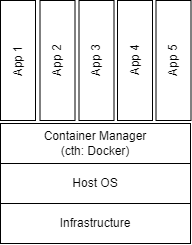
\includegraphics[width=.35\textwidth]{ContainerDiagram.png}
	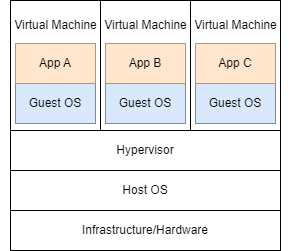
\includegraphics[width=.5\textwidth]{VirtualizationDiagram.png}
	\caption{Arsitektur Container vs Virtualization.}
	\label{fig:ContainerDiagram}
	\end{center}
\end{figure}

\section{Definisi}

\textbf{Container Architecture} merupakan sebuah konsep arsitektur yang dirancang untuk menjalankan aplikasi dalam container. Container Architecture memiliki beberapa tugas yaitu Isolasi, Portabilitas, Efisiensi, Deployment.

\textbf{Container} adalah metode menjalankan aplikasi yang memungkinkannya berjalan secara konsisten di berbagai lingkungan komputasi.\\ 
Secara sederhana, container dapat dianggap sebagai paket yang berisi semua elemen yang diperlukan untuk menjalankan aplikasi tertentu, seperti OS, library, config, dependencies, dan file penting lainnya yang dibutuhkan untuk menjalankan aplikasi tersebut.

\textbf{Docker} adalah platform open source untuk mengembangkan, menguji, dan mengimplementasikan aplikasi dalam container. 
Dalam konteks Docker, container adalah lingkungan terisolasi yang dapat berjalan di host yang sama tanpa pengaruh aplikasi atau sistem operasi lain yang berjalan di host yang sama. Container dapat dianggap sebagai paket yang berisi semua elemen yang diperlukan untuk menjalankan aplikasi tertentu, termasuk perangkat lunak, pustaka, konfigurasi, dan dependensi lainnya.

\textbf Alternatifnya {Kubernetes}, adalah platform open source untuk mengelola aplikasi dalam container yang dibuat oleh Google. Kubernetes memungkinkan pengguna untuk menjalankan, mengelola, dan mengotomatiskan penerapan aplikasi dalam container secara efisien.

\begin{figure}[h]
    \centering
    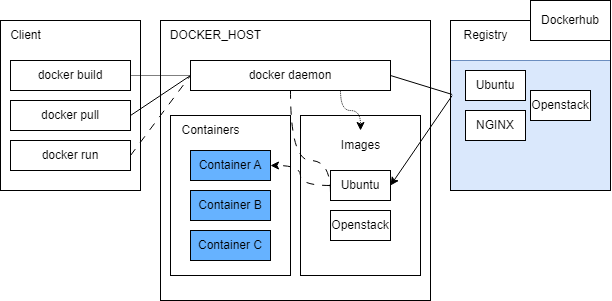
\includegraphics[width=\textwidth]{DockerDiagram.png}
    \caption{Diagram Docker.}
    \label{fig:ContainerDiagram}
\end{figure}

\textbf{Docker image}. Image disini bukan lah Image yang kita bayangkan (.jpg, .png, etc). Image pada Docker adalah sebuah template read-only atau cuplikan/snapshot berisikan instruksi untuk membuat container yang nantinya akan dipakai. Docker Image membuat Container untuk dijalankan di Docker Platform. Analoginya, Docker image itu seperti blueprint apartemen. 

\textbf{Docker Build}. Cara membuat Docker image adalah dengan membuat file Dockerfile (yaitu instruksi pembuatan imagenya) dan menggunakan "docker build" pada dockerfile tersebut. 

\textbf{Docker Pull} adalah perintah untuk mendownload/pull image docker dari registry(cth Dockerhub)

\textbf{Docker Registry} adalah sebuah repository berbagai docker images yang dibagikan oleh para developer.

\textbf {Docker Run} adalah perintah untuk menjalankan docker images dan membentuk Docker Container berdasarkan image yang dipilih.

\textbf {Docker Container} adalah instansi Container hasil dijalankannya image yang bisa distart, stop, restart, ataupun dihapus. Analoginya, inilah ruangan Kos apartemen hasil blueprint.

\textbf {Docker Daemon} adalah mesin/engine yang berjalan di mesin host dan memanage semua proses pada docker. Semua perintah perintah diatas seperti docker run itu dikirim ke docker daemon dan dijalankan.

\section{Kelebihan dan Kekurangan}
Berikut adalah kelebihan dan kekurangan docker:


\subsection{Kelebihan}
Keuntungan dari menggunakan docker adalah:
\begin{itemize}
\item Docker mempunyai konfigurasi yang \textit{sederhana} yang dapat disesuaikan dengan kebutuhan aplikasi yang sedang dikembangkan. Dengan menetapkan beberapa baris kode yang mendukung, docker mampu membuat lingkungannya sendiri yang terpisah dari lingkungan server utama.
\item Docker memiliki tingkat keamanan yang baik. Ia akan memastikan aplikasi yang sedang berjalan tidak dapat memengaruhi container \textit{(isolation)}. Selain itu, ia juga memiliki fitur keamanan \textit{pengaturan OS host mount} dengan akses \textit{read-only} sehingga konfigurasi yang tersedia tidak akan berubah sama sekali (kecuali pengguna memiliki akses penuh).
\item Docker dapat dijalankan pada beberapa platform cloud. Karena itu, pengguna dapat melakukan porting aplikasi dengan lebih mudah dan fleksibel. Selain itu, fitur-fitur docker juga dapat dijalankan pada berbagai sistem operasi, seperti Windows, Mac, dan Linux.
\item Docker mempunyai ukuran yang cukup ringan, dan lebih hemat sumber daya. Pengguna tidak membutuhkan memory storage atau overhead yang terlalu besar untuk menggunakannya.
\item Docker memiliki fitur debugging. Waktu yang dibutuhkannya juga tergolong cepat, yakni hanya sekitar satu menit saja untuk melakukan proses debug pada Sandbox.
\end{itemize}

\subsection{Kekurangan}
Konsekuensi dari menggunakan docker adalah sebagai berikut:
\begin{itemize}
\item Walaupun dapat digunakan pada berbagai macam OS, docker mempunyai kompatibilitas \textit{cross-platform} yang kurang fleksibel. Ketika sebuah aplikasi dirancang menggunakan Windows, pengguna memerlukan bantuan \textit{tools} eksternal untuk menjalankannya di Linux.
\item Secara garis besar, docker memiliki kekurangan fitur yang harus diakali pengguna dengan cara meng-install perangkat lunak eksternal apabila pengguna tidak ingin melakukan manajemen manual. Contohnya, docker tidak mempunyai dukungan untuk health-check, atau pemrograman ulang otomatis dari node yang tidak aktif.
\end{itemize}

\section{Contoh Kasus Penggunaan Container Architecture}

Biasanya, Container Architecture ergo Docker Container dibutuhkan dalam pembuatan dan deploy aplikasi yang terdiri dari beberapa komponen berbeda, seperti {aplikasi web} yang terdiri dari server web, database, dan layanan lainnya.

Dengan menggunakan Docker, kita dapat mengemas setiap komponen aplikasi ke dalam container yang terisolasi dan dapat dijalankan secara independen di berbagai lingkungan, seperti lingkungan pengembangan, pengujian, dan produksi. Container Docker memungkinkan pengembang untuk menjamin bahwa aplikasi yang mereka kembangkan dapat dijalankan dengan konsisten di seluruh lingkungan, sehingga mengurangi risiko terjadinya kesalahan dan masalah ketika aplikasi dideploy.

Tanpa container/docker, dalam pembuatan aplikasi kita biasanya harus install dan konfigurasi setiap komponen aplikasi secara manual di setiap environment, seperti environment pengembangan, pengujian, dan produksi. Ini bisa bermasalah ketika aplikasi dideploy di lingkungan yang berbeda, karena berbeda konfigurasi dan pengaturannya. 

\textbf{Contoh kasus}, misal ada sebuah aplikasi php yang sudah didevelop menggunakan php7, belum tentu aplikasi tersebut bisa dijalankan di komputer lain yang menjalankan php5. Dengan menggunakan docker, meskipun pada dasarnya komputernya menggunakan php5, namun image dan containernya sudah ada php7 jadinya tidak perlu konfigurasi ulang.

\section{Demo Container Architecture Menggunakan Docker}
Pada bagian ini Richwen akan mendemokan cara kerja docker. Codenya ada di folder code chapter 13.



\chapter{Pendahuluan}
\chapterauthor{Alfa Yohannis, Charlie Chaplin}

\section{Materi}
\begin{enumerate}
\item Introduction
\item Client-Server Architecture
\item Monolith vs. Distributed Architecture
\item Model-View-Controller Architecture
\item Layered Architecture
\item Event-Driven Architecture
\item Pipeline / Pipe-and-Filter Architecture
\item Service-based (Serverless) Architecture
\item Microkernel Architecture
\item Space-based Architecture
\item Orchestration-driven Service-oriented Architecture
\item Microservices Architecture
\item Containers
\item DevOps
\end{enumerate}




\backmatter
\addcontentsline{toc}{chapter}{Daftar Pustaka}
\bibliographystyle{splncs}
\bibliography{references}

\end{document}